\documentclass[11pt]{scrartcl} 


\usepackage{graphicx,graphics,tikz,pgfkeys}
\usetikzlibrary{arrows,decorations.pathreplacing}
\usepackage{amsmath}
\usepackage{amsthm}
\usepackage{amsfonts}
\usepackage{amssymb}
\usepackage{gensymb}



\usepackage{fixltx2e} % to be able to use the command \textsubscript

\usepackage[amssymb,thinqspace,textstyle,binary,noams,derivedinbase,derived]{SIunits} % To use SI units.
% amssymb: This option redefines the amssymb command \square to get
% the desired SIunits definition of the command.  Note: When using
% this option, the amssymb command \square can not be used.

%thinqspace This mode provides the use of \, (thin math space) as spacing be-
%        tween numerical quantities and units.

% textstyle:  When using the option textstyle units are printed in the typeface of the
%enclosing text, automatically.

%binary   This option loads the file binary.sty, which defines prefixes for binary
%         multiples.
%noams This option redefines the \micro command; use it when you don’t have
%         the AMS font, eurm10.
%derivedinbase This mode provides the ready-to-use expressions of SI derived units
%         in SI base units, e. g. \pascalbase to get ‘m−1 kg s−2 ’.
%derived This mode provides the ready-to-use expressions of SI derived units in SI
%         derived units, e. g. \derpascal to get ‘N m−2 ’.


%\usetikzlibrary{arrows,decorations.pathmorphing,backgrounds,placments,fit}
\usepackage[graphics,tightpage,active]{preview}
\PreviewEnvironment{tikzpicture}
\newlength\imagewidth
\newlength\imagescale

\begin{document}

sdssss\pgfmathsetlength{\imagewidth}{20cm} % desired displayed width of image
\pgfmathsetlength{\imagescale}{\imagewidth/1200} % pixel width of image
% adjust scale of tikzpicture (and direction of y) such that pixel
% coordinates can be used for drawing overlays:


\begin{center}
\begin{tikzpicture}[font=\sffamily]


  
  \begin{scope}[xshift=-2.5cm]
  \node[anchor=west,inner sep=0pt,outer sep=0pt] at (0cm,0cm)
{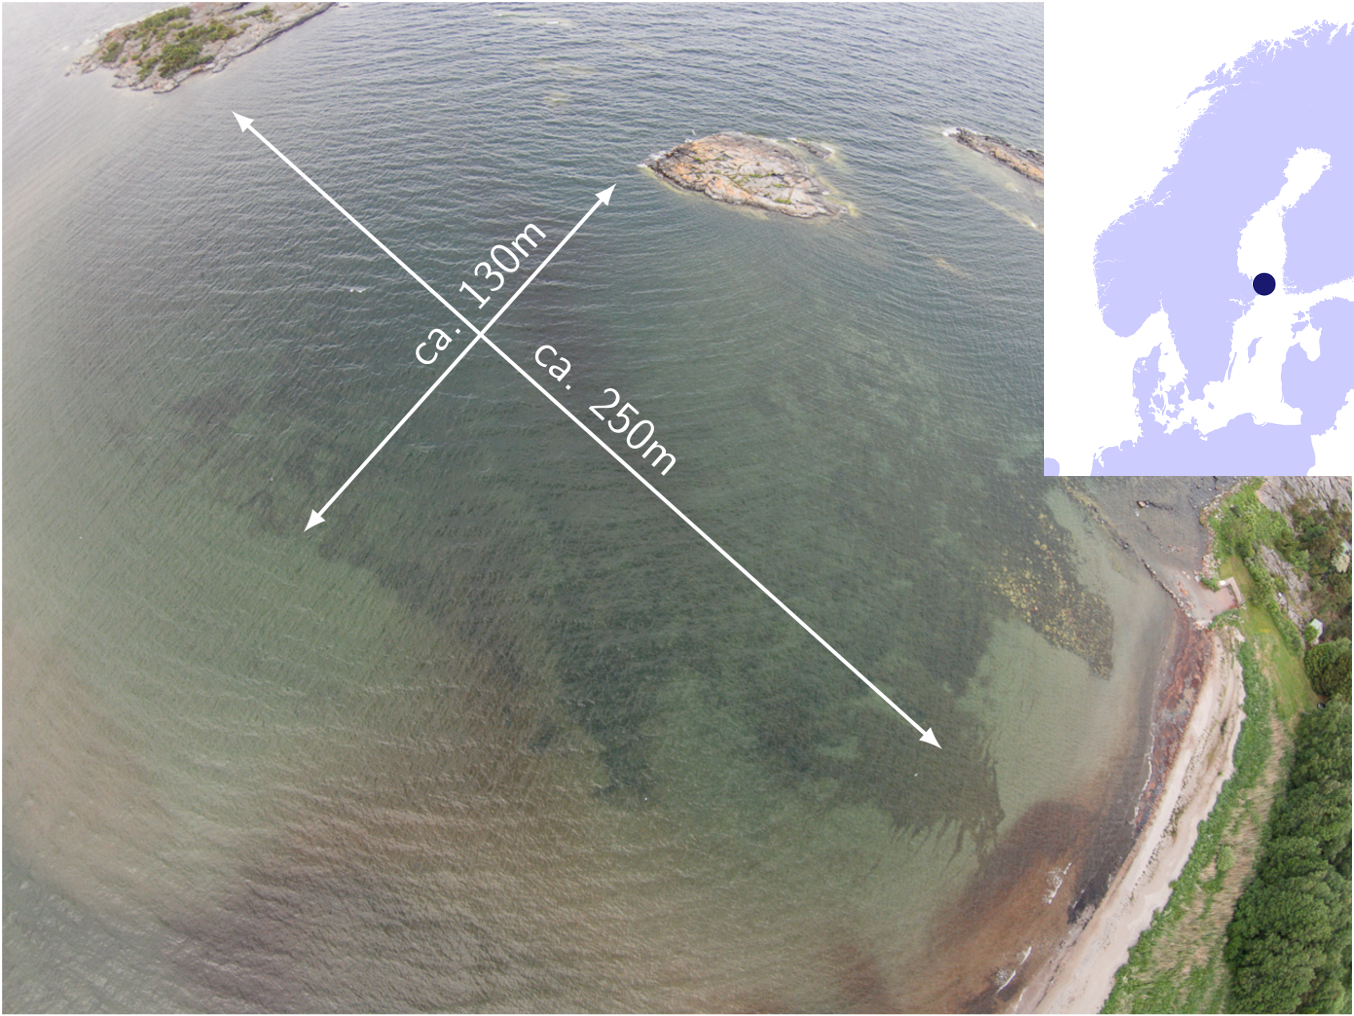
\includegraphics[trim=20 25 0 0,clip,width=2cm]{/home/alj/Dropbox/Presentations/2018ESEBMontpellier/images/BlogFigureHinderbengtsvikenMAP.png}};
\end{scope}
% Heat wave curve

\begin{scope}[yshift=-0.2cm]
% Axes
\node [scale=0.22] at (0.7cm,0.7cm) {Heat wave simulation};
\draw [-latex,line width=0.01cm] (0cm,0cm) -- node [scale=0.22,below=0.9cm]{Sampling times (weeks)} (1.5cm,0cm);
\draw [-latex,line width=0.01cm] (0,0cm) -- node [left=0.3cm,scale=0.22,rotate=90,anchor=north]{Temperature (\celsius)} (0cm,0.7cm);

%Temperature curve
% Controls:

\draw[color=red](0.01cm,0.06cm) -- (0.1cm,0.06cm)--
(0.2cm,0.4cm) -- (0.6cm,0.4cm)--
(0.7cm,0.06cm) -- (1.4cm,0.06cm);

%\draw[color=blue](0.01cm,0.05cm) -- (1.4cm,0.05cm);

% Sampling times
\draw[color=black,line width=0.007cm] (0.1cm,-0.05cm) -- node [scale=0.22,below=1.4cm]{0} (0.1cm,0.5cm);
\draw[color=black,line width=0.007cm] (0.6cm,-0.05cm) -- node [scale=0.22,below=1.4cm]{3} (0.6cm,0.5cm);
\draw[color=black,line width=0.007cm] (1.2cm,-0.05cm) -- node [scale=0.22,below=1.4cm]{8} (1.2cm,0.5cm);

%\draw [latex] (-2cm,8cm) -- (0cm,8cm) -- (1cm,12cm) -- (2cm,16cm) -- (3cm,20cm) --
%(4cm,24cm) -- (14cm,24cm) -- 
%(15cm,20cm) -- (16cm,16cm) -- (17cm,12cm) -- 
%(18cm,8cm)-- (28cm,8cm);

% Axis ticks
\draw (0cm,0.05cm) -- node [left=.02cm,scale=0.22] {15} (-0.05cm,0.05cm);
%\draw (-2.2cm,12cm) -- node [left=.2cm,text size=0.3] {12\celsius} (-3.2cm,12cm);
%\draw (-2.2cm,16cm) -- node [left=.2cm,text size=0.3] {16\celsius} (-3.2cm,16cm);
%\draw (-2.2cm,20cm) -- node [left=.2cm,text size=0.3] {20\celsius} (-3.2cm,20cm);
\draw (0cm,.4cm) -- node [left=.02cm,scale=0.22] {27} (-0.05cm,0.4cm);

%\draw (0cm,7cm) -- node [below=.2cm,text size=0.3] {0d} (0cm,6cm);
%\draw (4cm,7cm) -- node [below=.2cm,text size=0.3] {4d} (4cm,6cm);
%\draw (6cm,7cm) -- node [below=.2cm,text size=0.3] {6d} (6cm,6cm);
%\draw (14cm,7cm) -- node [below=.2cm,text size=0.3] {14d} (14cm,6cm);
%\draw (18cm,7cm) -- node [below=.2cm,text size=0.3] {18d} (18cm,6cm);
%\draw (28cm,7cm) -- node [below=.2cm,text size=0.3] {28d} (28cm,6cm);



\end{scope}
\node [scale=0.4,color=white] at (-2.4cm,0.6cm) {a)};
  \node [scale=0.4,color=black] at (-0.3cm,0.6cm) {b)};

\end{tikzpicture}


\end{center}

\end{document}